It was previously observed that the mass resolution in Monte Carlo deteriorated for displaced vertices. The problem arises due to the track parameters not being adjusted for the vertex position~\cite{billoir_fast_1992}. A correction to the measured mass is defined as shown in Figure~\ref{eq:massCorrection}.

\begin{equation}
\label{eq:massCorrection}
m_{corr} = m_{uc} - \dfrac{0.15\times 10^{-3}\times z_{vtx}}{m_{uc}}(\dfrac{P_{x,e-}}{P_{e-}}-\dfrac{P_{x,e+}}{P_{e+}})            
\end{equation}

In Equation~\eqref{eq:massCorrection}, the unconstrained vertex mass is $m_{uc}$, the reconstructed $z$ vertex position downstream is $z_{vtx}$, the horizontal momentum component is indicated by $P_x$ where the corresponding particle type is also indicated by the subscript, and the magnitude of the momentum is $P$. The effects of the correction to the reconstructed mass can be seen in Figure~\ref{fig:effectMCorr}.

\begin{figure}[H]
  \centering
      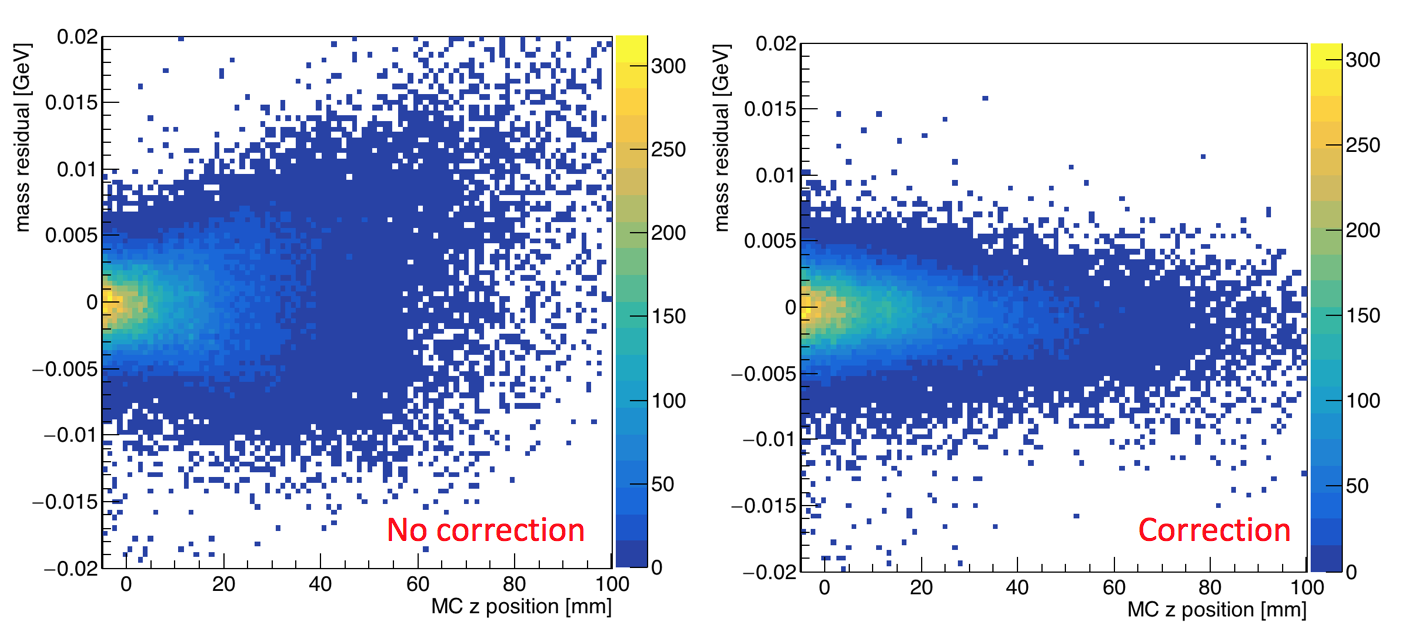
\includegraphics[width=0.9\textwidth]{pics/searching/massCorrection.png}
  \caption[Correction to the reconstructed mass for a 40~MeV A$^{\prime}$]{The mass residual of a reconstructed 40~MeV A$^{\prime}$ is shown as a function of vertex position in $z$. The uncorrected mass residual as given from the vertexer is shown on the left. The resolution deteriorates with the downstream $z$ position of the vertex. After the correction is applied, as shown on the right, the mass resolution is no longer vertex position dependent.}
  \label{fig:effectMCorr}
\end{figure} 

The mass resolution is determined from A$^{\prime}$ Monte Carlo and has been checked with the $e-e-$ mass resolution from M\o ller scattered electron pairs in data. By generating heavy photons at discrete masses, applying the cuts proposed in data, and fitting the A$^{\prime}$ mass peak residual with respect to the generated mass peak, the mass resolution can be measured as a function of mass. A fit to the generated 40~MeV heavy photon in Monte Carlo is shown in Figure~\ref{fig:ap40mev}.

\begin{figure}[H]
  \centering
      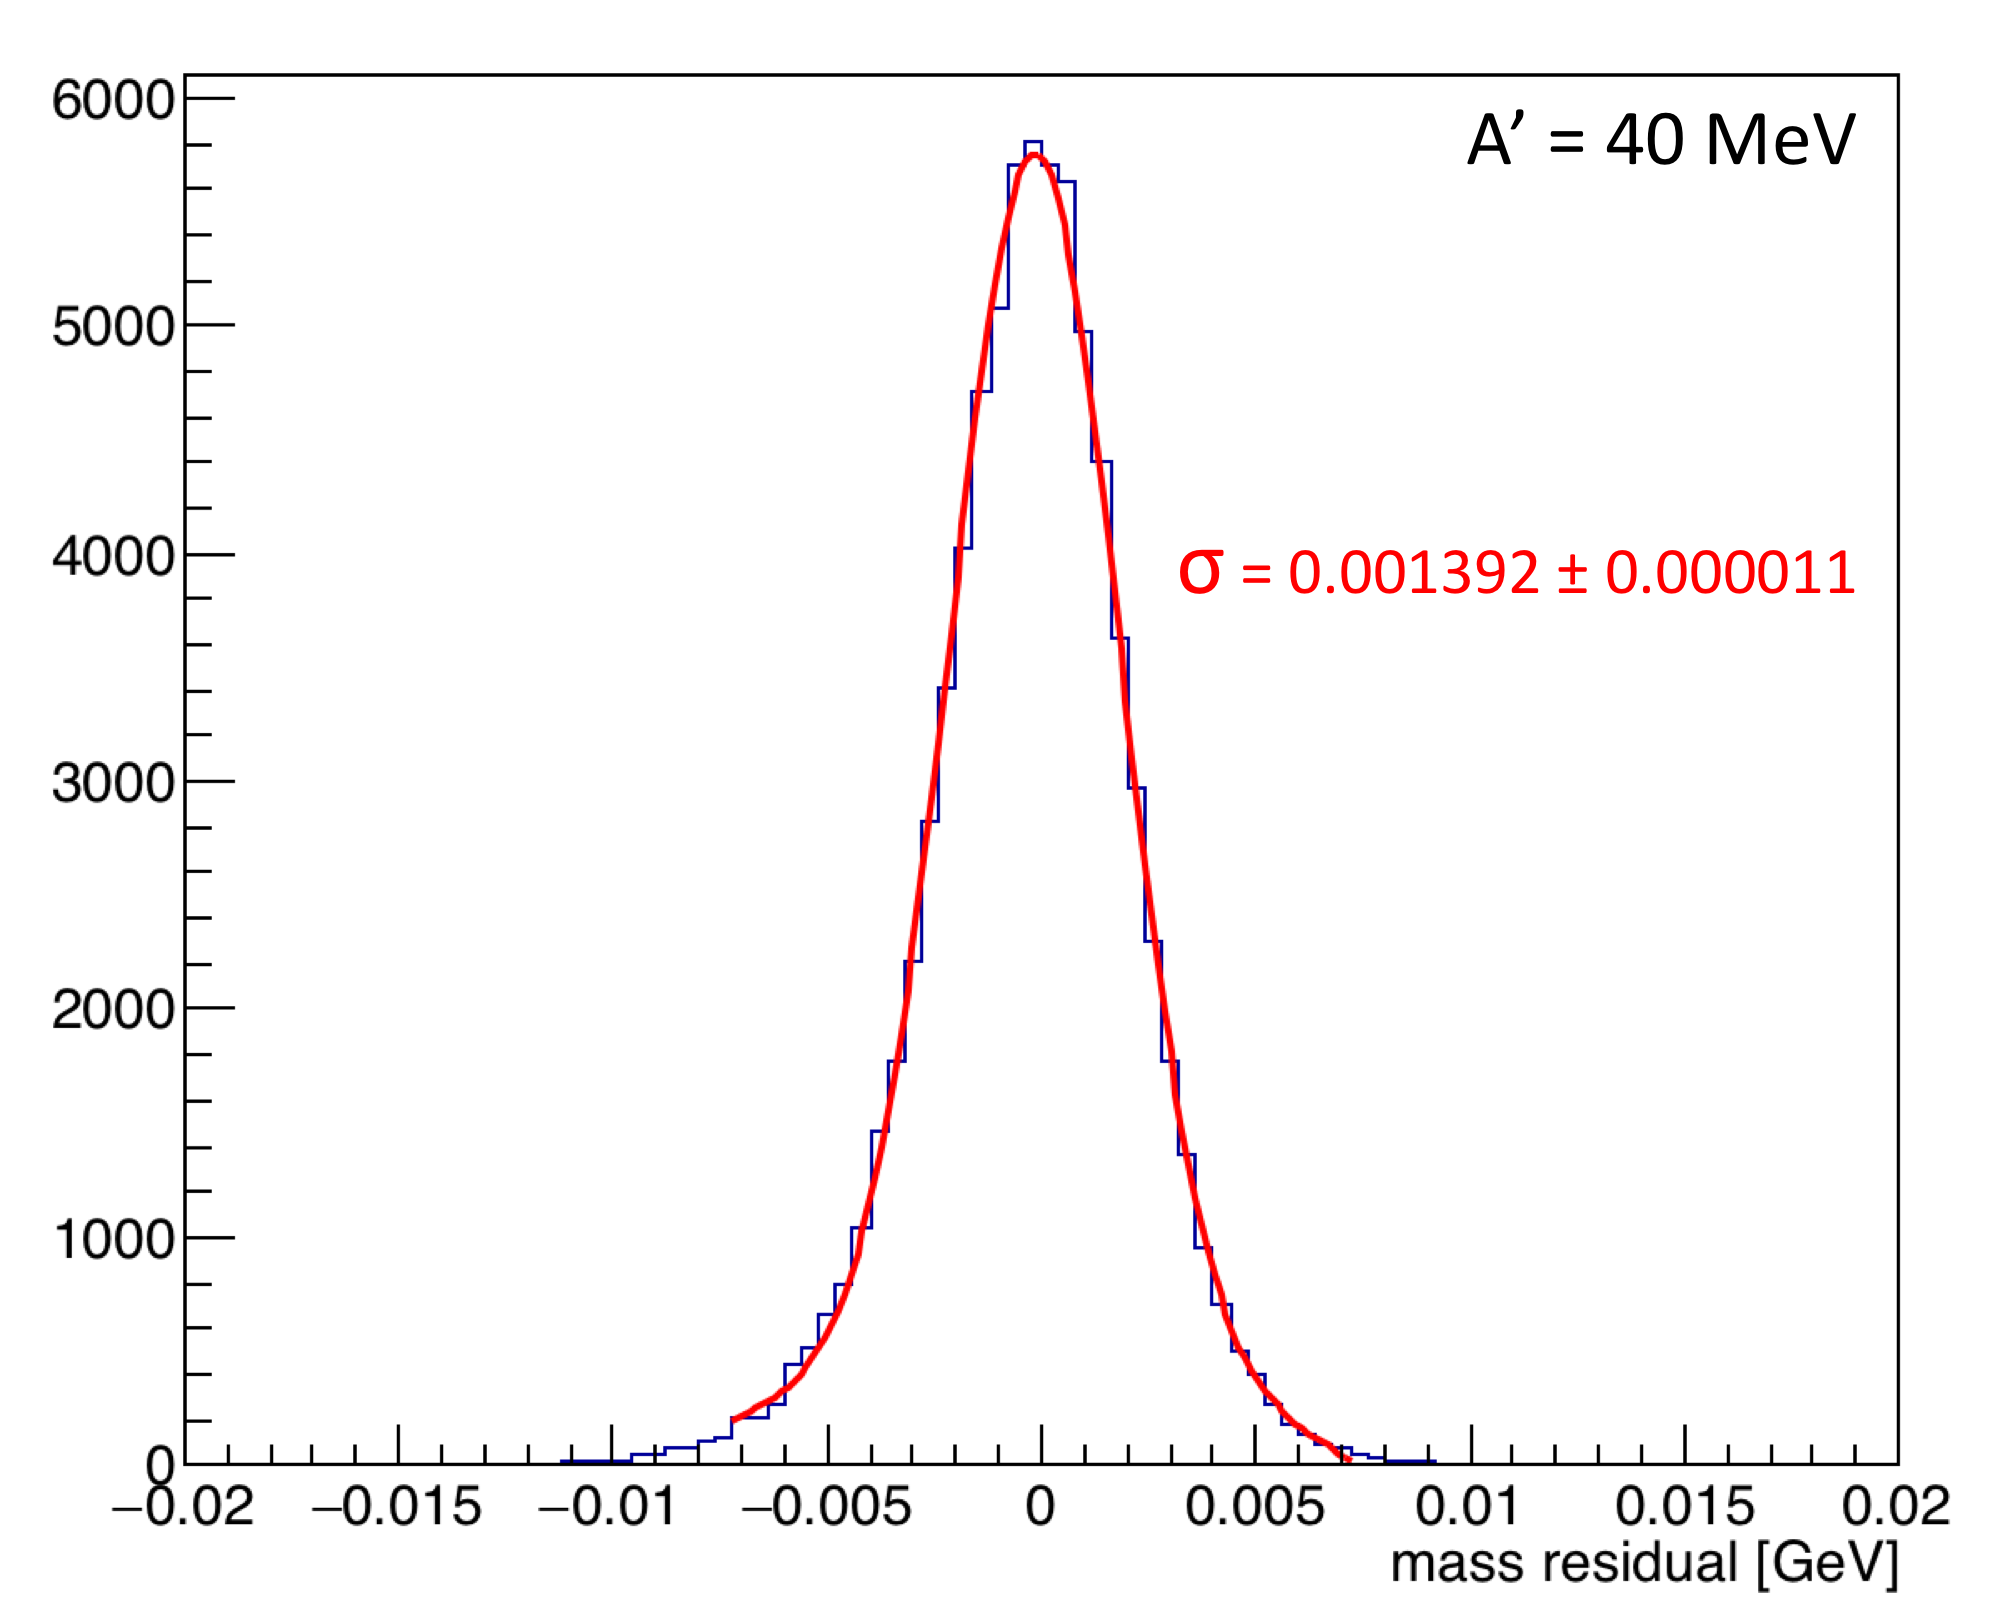
\includegraphics[width=0.9\textwidth]{pics/searching/ap40mev.png}
  \caption[Fit to the mass residual of a 40~MeV A$^{\prime}$]{The residual of a reconstructed 40~MeV A$^{\prime}$ mass is shown with a Gaussian fit.}
  \label{fig:ap40mev}
\end{figure} 

Simulations of the M\o ller mass can be used to study systematic offsets between the measured mass resolution in data and the mass resolution found in Monte Carlo. Using M\o ller Monte Carlo (with no beam background), the Moller mass can be seen in Figure~\ref{fig:mollerMC}. 

\begin{figure}[H]
  \centering
      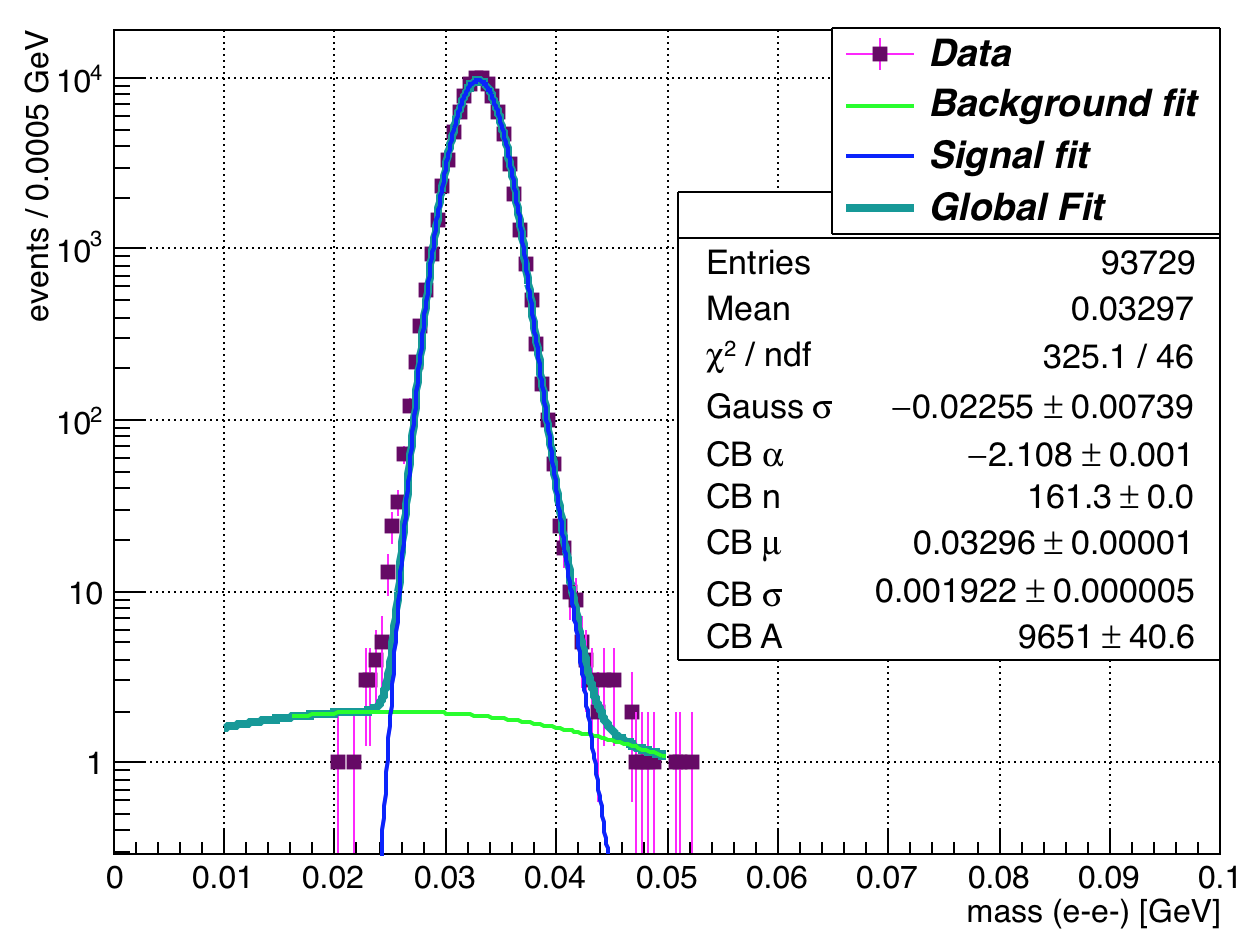
\includegraphics[width=0.9\textwidth]{pics/searching/mollerMassMC.png}
  \caption[Fit to the M\o ller mass peak in Monte Carlo]{The M\o ller mass peak from Monte Carlo with a Crystal Ball fit is shown. The background is fit with a Gaussian.}
  \label{fig:mollerMC}
\end{figure} 

The M\o ller mass from Monte Carlo can be immediately compared with the M\o ller mass found in data. The difference in resolution between the peak from the pure Monte Carlo M\o ller sample and the M\o ller sample in data is approximately 17$\%$. This difference should be applied to the heavy photon mass resolution found in Monte Carlo in order to appropriately scale the bin widths when slicing and fitting the vertex distribution by mass. The M\o ller peak from data is shown in Figure~\ref{fig:mollerMass}. 

\begin{figure}[H]
  \centering
      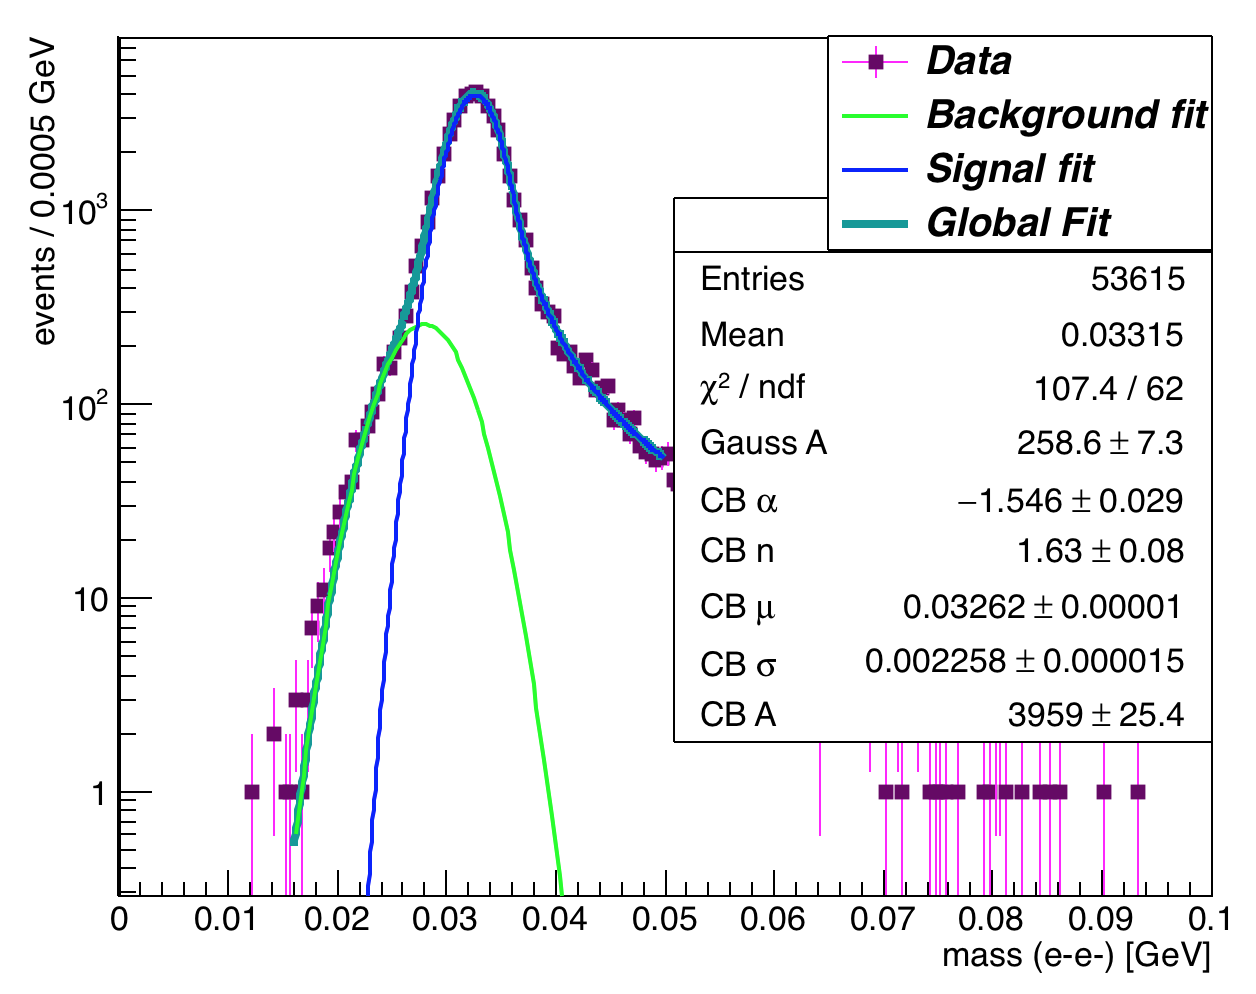
\includegraphics[width=0.9\textwidth]{pics/searching/mollerMass.png}
  \caption[Fit to the M\o ller mass peak in data]{The M\o ller mass peak with a Crystal Ball fit in data is shown.The low mass background on the front of the peak is fit with a Gaussian.}
  \label{fig:mollerMass}
\end{figure} 

The mass resolution is shown on Figure~\ref{fig:massRes} as a function of mass.

\begin{figure}[H]
  \centering
      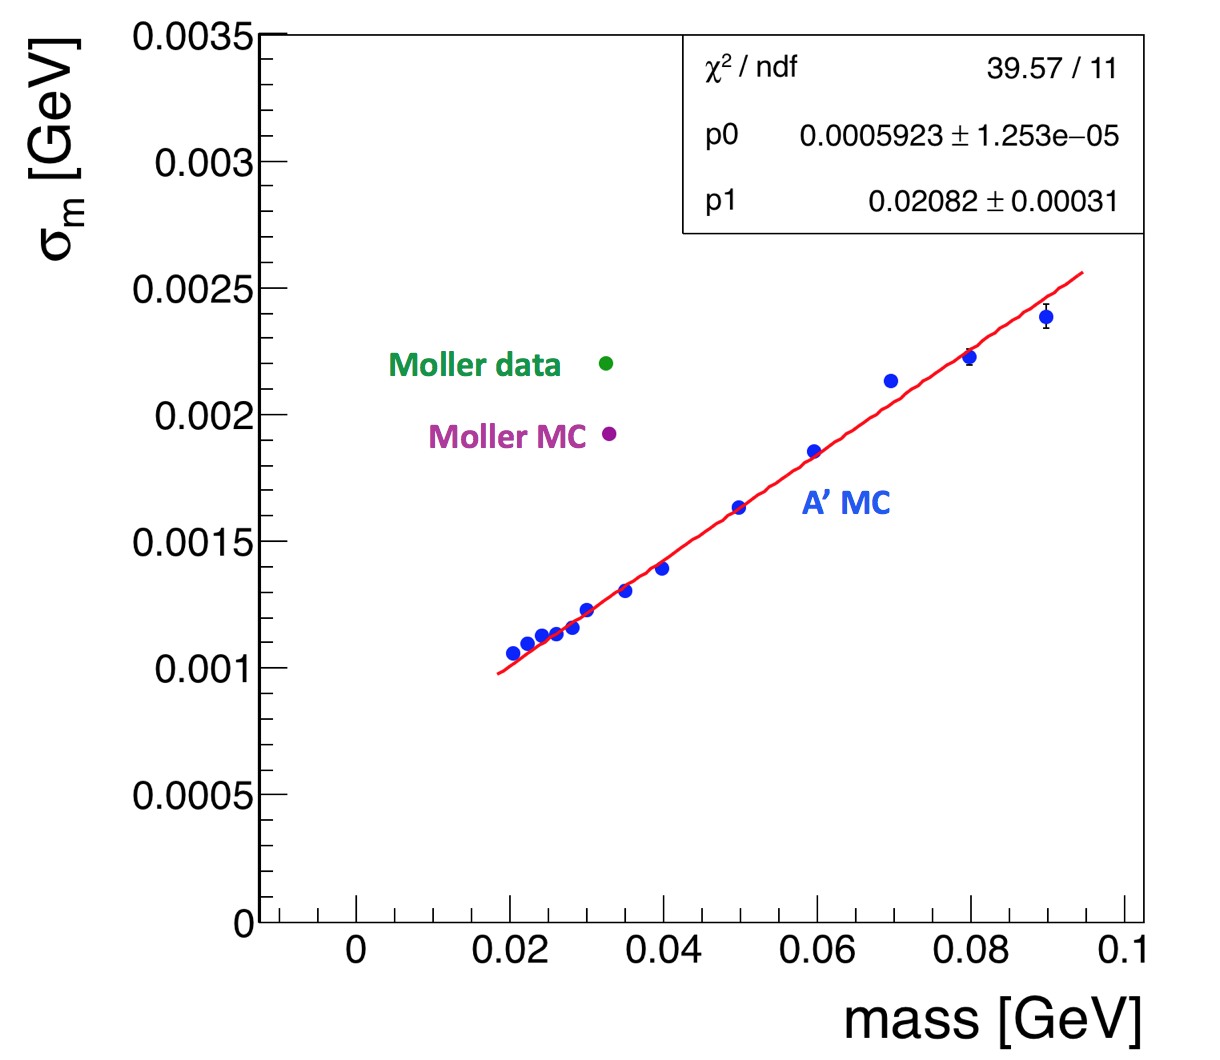
\includegraphics[width=0.9\textwidth]{pics/searching/massResolution.png}
  \caption[Mass resolution compared between Monte Carlo and data]{The mass resolution is compared here between Monte Carlo and data. The mass resolution points shown in blue measure the residual of the reconstructed mass in heavy photon Monte Carlo. The mass resolution shown in purple is from the fit to the Moller mass peak when reconstructed in Monte Carlo. The green point is the Moller mass resolution as measured in data. The difference between the Monte Carlo and data Moller mass resolutions is approximately 17$\%$. This scaling should be applied to the linear fit $0.02082m+0.0006$ from Monte Carlo in order to account for the difference in resolution.}
  \label{fig:massRes}
\end{figure} 

After applying the 17$\%$ scaling to the mass resolution from A' Monte Carlo, we obtain the mass resolution in Equation~\eqref{eq:massresScaled}.

\begin{equation}
\label{eq:massresScaled}
\sigma_m = 0.02082m+0.0007
\end{equation}

The scaled mass resolution in Equation~\eqref{eq:massresScaled} is used in the vertex analysis to find the $z$ vertex cut. 



